\documentclass[10pt,letterpaper]{article}
\usepackage[utf8]{inputenc}
\usepackage[margin=1in]{geometry}
\usepackage{amsmath}
\usepackage{amsfonts}
\usepackage{amssymb}
\usepackage{graphicx}
\usepackage{hyperref}
\usepackage{listings}
\usepackage{color}

\definecolor{codegreen}{rgb}{0,0.6,0}
\definecolor{codegray}{rgb}{0.5,0.5,0.5}
\definecolor{codepurple}{rgb}{0.58,0,0.82}
\definecolor{backcolour}{rgb}{0.95,0.95,0.92}

\lstdefinestyle{mystyle}{
    backgroundcolor=\color{backcolour},   
    commentstyle=\color{codegreen},
    keywordstyle=\color{magenta},
    numberstyle=\tiny\color{codegray},
    stringstyle=\color{codepurple},
    basicstyle=\footnotesize,
    breakatwhitespace=false,         
    breaklines=true,                 
    captionpos=b,                    
    keepspaces=true,                 
    numbers=left,                    
    numbersep=5pt,                  
    showspaces=false,                
    showstringspaces=false,
    showtabs=false,                  
    tabsize=4
}

\lstset{style=mystyle}

\title{Quarter 4 Physics Project - Kinematics}
\date{\today}
\author{Bhaskar Mishra}

\begin{document}
    \maketitle
    \pagenumbering{gobble}
    \newpage
    \tableofcontents
    \newpage
    \pagenumbering{arabic}
    
    \section{Background Knowledge}
    
    Since we are solving a kinematics problem, there are various formulas and points that will likely be useful in solving this problem. For example, the following relationships between position, velocity, and acceleration:
    \begin{align*}
    	\frac{\textrm{d}x}{\textrm{d}t}&=v(t)\\
       	\frac{\textrm{d}v}{\textrm{d}t}&=a(t)\\
    \end{align*}
    In addition to this information, a quick glance at the problem makes it apparent that the impulse-momentum relationship will also play a vital role in the problem. Here's the formula:
    \begin{equation*}
    	F\Delta t = m\Delta v
    \end{equation*}
    Finally, there are the standard physics formulas and definitions that will likely be useful:
    \begin{align*}
    	F&=ma\\
    	F_{\textrm{friction}}&=\mu \cdot F_N\\
    	1\:\textrm{MN} &= 1\times 10^6\: \textrm{N}\\
    \end{align*}
    
   	\section{Analysis}
   	
   	This problem is structured in a way that it begs to be solved backwards. In this paper, we'll be doing just that, starting with the sub-problem used to calculate the time the force is applied.
   	
   	\subsection{Vehicle Friction Sub-Problem}
   	
   	\begin{figure}[h!]
   		\centering
   		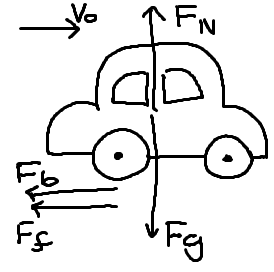
\includegraphics[scale=0.5]{CarFBD1.png}
   		\caption{Vehicle Free Body Diagram}
   		\label{fig:carfbd1}
   	\end{figure}
   	
   	For the Vehicle Friction Sub-Problem, we are given a couple of variables:
   	
   	\begin{align*}
   		\textrm{Mass of Vehicle}=M&=1500\:\textrm{kg}\\
   		\textrm{Coefficient of Friction}=\mu&=0.38\\
   		\textrm{Initial Velocity}=v_0&=45\:\textrm{mph}=20.1168\:\textrm{m/s}\\
   		\textrm{Braking Force}=F(v)&=0.27v^3\\
   	\end{align*}
   	
   	Using these variables, we have to calculate the time it takes the vehicle to come to rest. First, we need to calculate the net horizontal force experienced by the vehicle. As shown in Figure~\ref{fig:carfbd1}, this is equal to negative the sum of the braking force and the frictional force acting on the car:
   	
   	\begin{align*}
   		\sum F_x &= -(F_b+F_f)=-(0.27v^3+\mu \cdot F_N)\\
   	\end{align*}
   	
   	This is dependent on $F_N$, which can be calculated by applying Newton's Second Law on vertical forces.
   	\begin{align*}
   		\sum F_y &= F_N-F_g\\
   		&= F_N-Mg=0\\
   		F_N &= Mg
   	\end{align*}
   	
   	Plugging this back into the original equation, we get the following:
   	\begin{equation*}
		Ma_x=-0.27v_x^3-\mu Mg
   	\end{equation*}
   	
	Solving for $a_x$:
	\begin{equation*}
		a_x=\frac{\textrm{d}v_x}{\textrm{d}t} = \frac{-0.27v_x^3}{M}-\mu g
	\end{equation*}
	
	Now the issue here is that this differential equation is not one that can easily be solved for a closed form function of time to represent $v_x$. As a result of this, we will resort to computational methods to solve this. We'll assume constant acceleration over small $dt$'s and use the equation $v_f=v_i+a\cdot \Delta t$ to update velocity. Once velocity becomes negative, we'll store the value of time as the time it takes for the vehicle to come to a stop. This will be done in the Calculations section later on in this paper.
	
	\subsection{Impulse-momentum Sub-Problem}
	
	For this problem, we now need to use the time calculated in the previous section along with the impulse-momentum relationship:
	\begin{align*}
		F\Delta t &= m\Delta v\\
		\Delta v &= F\Delta t/m
	\end{align*}
	We will assume that the velocity along the z-axis of the particle prior to experiencing the force was 0. With this we get the following equation for initial velocity:
	\begin{align*}
		v_{z0} &= \frac{F\Delta t}{m}\\
	\end{align*}
	
	\subsection{Particle Simulation Sub-Problem}
	
	Finally, using the same method used in the Vehicle Friction Sub-Problem, we'll assume constant acceleration for small $dt$'s and use computational methods to simulate the motion of the problem. As before, this will be done in the Calculations section of this paper.
	
	\section{Assumptions}
	
	Before moving on to the Calculations section of this paper, I'd like to create a list of any assumptions I've made during this problem:
	\begin{itemize}
		\item Our greatest assumption is the assumption that acceleration will be constant over small units of time. This assumption will likely create some error in our solution, but it shouldn't be too significant if we choose to use a small $dt$. For the purposes of this problem, we will likely use a $dt$ between $0.0001$ and $0.001$.
		\item We also make the typical assumption of zero air-resistance. The error generated by this assumption shouldn't be significant, and including this in our calculations would complicate things a lot as vehicles have very complex shapes.
		\item For the sake of this problem, we will be assuming that all the problems are taking place near the surface of the earth. This allows us to have a constant acceleration due to gravity of about $9.80665\:m/s^2$ (\href{https://nvlpubs.nist.gov/nistpubs/Legacy/SP/nistspecialpublication330e2008.pdf}{Source}). We will use the approximation $9.81\:m/s^2$ for the rest of this paper.
		\item In terms of problem interpretation assumptions we have two significant assumptions. One, we assume that $v_z$ function is equal to the $v_{z0}$ calculated in the Impulse-momentum Sub-Problem for the time period from 0 to the time calculated in the Vehicle-Friction Sub-Problem and equal to the function provided for the rest of the time. Secondly, we also assume that the fourth root of $v_z$ in the calculation of z is taking the root of the magnitude of $v_z$.
	\end{itemize}
	
	\section{Calculations}
		\subsection{Vehicle Friction Sub-Problem}
		 	Here is the code for the problem:
		 	\begin{lstlisting}[language=Python]
def vehicle(dt):
	M = 1500
	mu = 0.38
	v = [20.1168]

	while v[-1] > 0:
		a = -0.27 * math.pow(v[-1], 3) / M - mu * g
		v.append(v[-1] + a * dt)

	return [dt * i for i in range(len(v))], v
			 \end{lstlisting}

			The vehicle function returns an array of times along with an array of velocities for each respective time. The function will keep generating values until the velocity is less than zero.
			With $dt = 0.001$, the last element of the time array is $t\approx \boxed{4.96 \textrm{ s}}$.
		\subsection{Impulse-momentum Sub-Problem}
			 Here is the code for the problem:
			 \begin{lstlisting}[language=Python]
def impulse_momentum(t):
	F = 1.51 * math.pow(10, 6)
	m = 10 * math.pow(10, -3)
	return F * t / m
			 \end{lstlisting}

			 Other than some basic conversions, this function just calculates the exact expression derived earlier. Using $t=4.96\textrm{ s}$ from earlier, this function gives us $v_{z0}\approx \boxed{748960000 \textrm{ m/s}}$ 
		\subsection{Particular Simulation Sub-Problem}
			 Here is the code for the problem:
			 \begin{lstlisting}[language=Python]
def final_problem(vz0, dt, t_im):
	vz = lambda z, t: vz0/3 - 7*z/(2*t) + 5 * math.pow(t, 2/3) if t > t_im else vz0
	z = lambda vz, x, y, t: -0.5*math.pow(x, 2) + math.pow(y, 0.5) + (3*x*vz*t/(2*y) if t > 0 else 0) - 2*math.pow(abs(vz), 1/4)
	y = lambda x, t: -math.pow(t, 2) + 3 * x * t
	x = lambda t: 2*math.pow(t, 3) - math.pow(t, 2) + 5*t
	vx = lambda t: 6*t*t-2*t+5
	vy = lambda t, x, vx: -2*t + 3*x + 3*t*vx

	t = [0]
	xi = [0]
	yi = [0]
	zi = [0]
	vzi = [0]
	vxi = [0]
	vyi = [0]
	while t[-1] < 10:
		xi.append(x(t[-1]))
		yi.append(y(xi[-1], t[-1]))
		vxi.append(vx(t[-1]))
		vyi.append(vy(t[-1], x[-1], vxi[-1]))
		vzi.append(vz(zi[-1], t[-1]))
		zi.append(z(vzi[-1], xi[-1], yi[-1], t[-1]))
		t.append(t[-1] + dt)

	return t, xi, yi, zi, vxi, vyi, vzi
			 \end{lstlisting}

			 As with previous problems, this uses small dt's to calculate the value of each variable at various times. Specifically, the function returns a time array with various times, and then 6 more arrays recording x-position, 
			 y-position, z-position, x-velocity, y-velocity, and z-velocity for the particle. The kinetic and potential energies of the particles are then calculated using their respective formulas ($KE=\frac{1}{2}mv^2$ and $PE=mgh$).
			 Once all the results are graphed, we get the following graphs:

			 \begin{figure}[h!]
				\centering
				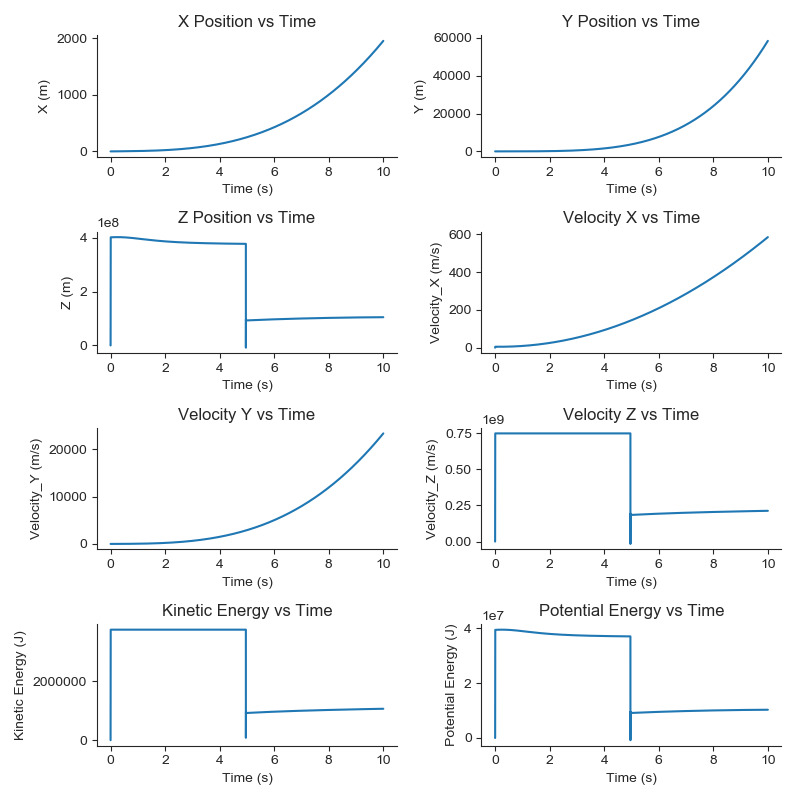
\includegraphics[scale=0.4]{Results.png}
				\caption{Graphs}
				\label{fig:graphs}
			\end{figure}
			\newpage
	\section{Final Thoughts}
		\subsection{Conclusion}
			Through the results calculated above, we can conclude that the particle's x and y position increases at an increasing rate whereas the z position decreases over time during the first 4.96 seconds and then increases afterwards.
		\subsection{Reflection}
			Though this project took a semester to complete, it was a true learning experience for me and I've developed many skills through its completion. For one, creating this paper required me to really solidify my LaTeX skills. I used
			many packages I had never used before and made many visual formatting changes I wouldn't usually make. In addition to the typesetting, this project also taught me a lot about data manipulation and data presentation in Python. I learned
			to use new libraries such as matplotlib, seaborn, and pandas that allowed me to manipulate large quantities of data and then visualize them in well-formatted graphs like the ones seen above. Finally, though I understood how using
			computational methods in physics worked before, this was the first actually implementing that kind of approach to solve a problem. It was definitely an interesting experience, and it required a much different thought process than just
			taking the derivative / integral of random functions. All in all, this project was a great learning experience, and I'm excited to use the knowledge I've gained in the many research papers I'll work on in the future.
\end{document}